% Options for packages loaded elsewhere
\PassOptionsToPackage{unicode}{hyperref}
\PassOptionsToPackage{hyphens}{url}
%
\documentclass[
]{article}
\title{Analysis/results Replication of Mani et al.~2013 - For Open
Science course}
\author{}
\date{\vspace{-2.5em}}

\usepackage{amsmath,amssymb}
\usepackage{lmodern}
\usepackage{iftex}
\ifPDFTeX
  \usepackage[T1]{fontenc}
  \usepackage[utf8]{inputenc}
  \usepackage{textcomp} % provide euro and other symbols
\else % if luatex or xetex
  \usepackage{unicode-math}
  \defaultfontfeatures{Scale=MatchLowercase}
  \defaultfontfeatures[\rmfamily]{Ligatures=TeX,Scale=1}
\fi
% Use upquote if available, for straight quotes in verbatim environments
\IfFileExists{upquote.sty}{\usepackage{upquote}}{}
\IfFileExists{microtype.sty}{% use microtype if available
  \usepackage[]{microtype}
  \UseMicrotypeSet[protrusion]{basicmath} % disable protrusion for tt fonts
}{}
\makeatletter
\@ifundefined{KOMAClassName}{% if non-KOMA class
  \IfFileExists{parskip.sty}{%
    \usepackage{parskip}
  }{% else
    \setlength{\parindent}{0pt}
    \setlength{\parskip}{6pt plus 2pt minus 1pt}}
}{% if KOMA class
  \KOMAoptions{parskip=half}}
\makeatother
\usepackage{xcolor}
\IfFileExists{xurl.sty}{\usepackage{xurl}}{} % add URL line breaks if available
\IfFileExists{bookmark.sty}{\usepackage{bookmark}}{\usepackage{hyperref}}
\hypersetup{
  pdftitle={Analysis/results Replication of Mani et al.~2013 - For Open Science course},
  hidelinks,
  pdfcreator={LaTeX via pandoc}}
\urlstyle{same} % disable monospaced font for URLs
\usepackage[margin=1in]{geometry}
\usepackage{graphicx}
\makeatletter
\def\maxwidth{\ifdim\Gin@nat@width>\linewidth\linewidth\else\Gin@nat@width\fi}
\def\maxheight{\ifdim\Gin@nat@height>\textheight\textheight\else\Gin@nat@height\fi}
\makeatother
% Scale images if necessary, so that they will not overflow the page
% margins by default, and it is still possible to overwrite the defaults
% using explicit options in \includegraphics[width, height, ...]{}
\setkeys{Gin}{width=\maxwidth,height=\maxheight,keepaspectratio}
% Set default figure placement to htbp
\makeatletter
\def\fps@figure{htbp}
\makeatother
\setlength{\emergencystretch}{3em} % prevent overfull lines
\providecommand{\tightlist}{%
  \setlength{\itemsep}{0pt}\setlength{\parskip}{0pt}}
\setcounter{secnumdepth}{-\maxdimen} % remove section numbering
\ifLuaTeX
  \usepackage{selnolig}  % disable illegal ligatures
\fi

\begin{document}
\maketitle

\hypertarget{r-markdown}{%
\subsection{R Markdown}\label{r-markdown}}

This is a document demonstrating how the analysis and results section of
the replication paper will be conducted. Everything is adapted from the
original Mani et al.~(2013) paper.

Three variables are added: the total\_iq\_score, a simple sum of the
number of correct answers in the iq test, and a priming, which
identifies if the participant saw the high (coded as 1) or low (coded as
0) priming. The last variable is whether the participant had a household
income, divided by the square root of the household size, above (1) or
below (0) the median income level (divided by household size) of the
sample. This was used in the original study as a proxy for if the
participants were ``poor'' or ``rich''.

In the original paper the main analysis of interest for the shopping
mall study was a two-way ANOVA so this is also used here, aov()-function
is used.

\% Error: Unrecognized object type.
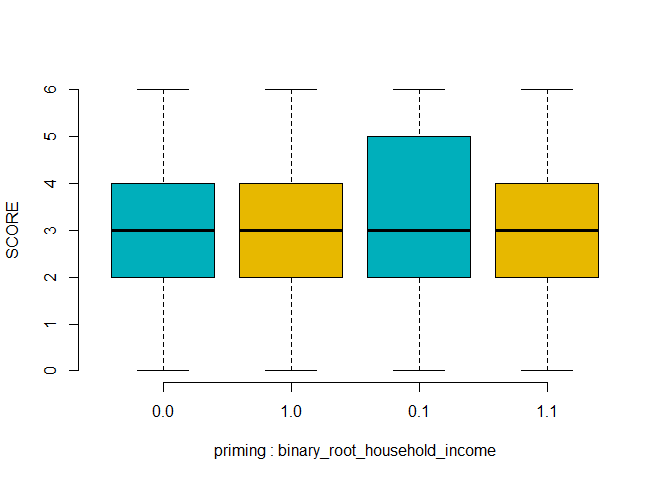
\includegraphics{Markdown-mani-et-al-replication_files/figure-latex/analysis-1.pdf}

\hypertarget{temporary-outline-ntoes}{%
\subsection{Temporary outline ntoes}\label{temporary-outline-ntoes}}

\hypertarget{introduction}{%
\subsection{Introduction}\label{introduction}}

We tried to replicate experiment 4 from study 1 in mani et al (poverty
impedes cognitive function) -- the shopping mall study where people read
each scenario and then responded to a IQ test. \#\# Methods We increased
the sample size to 500 and collected via prolific.co. Different from
original where they were collected in person in a shopping mall. Only
americans. Good spread of income level. \#\#\# Tests Not ravens matrices
but very similar -- hagen matrices. Six rounds increasing difficulty. We
note that this is different to original where they got 3 rounds randomly
selected.

\hypertarget{results}{%
\subsection{Results}\label{results}}

We found no effects in an anova.

\hypertarget{discussion}{%
\subsection{Discussion}\label{discussion}}

\begin{verbatim}
Perhaps something wrong with priming, perhaps it does not work. But it did in the original. Also - Bickel et al. (2016) managed to get effects with a somewhat similar priming (negative income shock in a short narrative text, participants asked to simply think about it for a while). This was on temporal discounting though, and not the IQ-effect described here.  IQ-effect probably not there. 
\end{verbatim}

\end{document}
